\begin{frame}
    \frametitle{Использованные технологии}
    \begin{itemize}
        \item Графическое API --- DirectX 12 как отраслевой стандарт
        \item Инструменты разработки --- Visual Studio
        и компилятор Microsoft Visual C++,
        т.к. они имеют официальную поддержку DirectX 12
        \item Отладчик графики --- PIX,
        поскольку он поддерживает DirectX 12
    \end{itemize}
\end{frame}

\begin{frame}
    \frametitle{Отрисовка загруженной из файла модели}
    \includegraphics[width=\textwidth]{images/base.png}
\end{frame}

\begin{frame}
    \frametitle{Шейдер пост-обработки}
    \includegraphics[width=\textwidth]{images/sobel.png}
\end{frame}

\begin{frame}
    \frametitle{Отрисовка нормалей}
    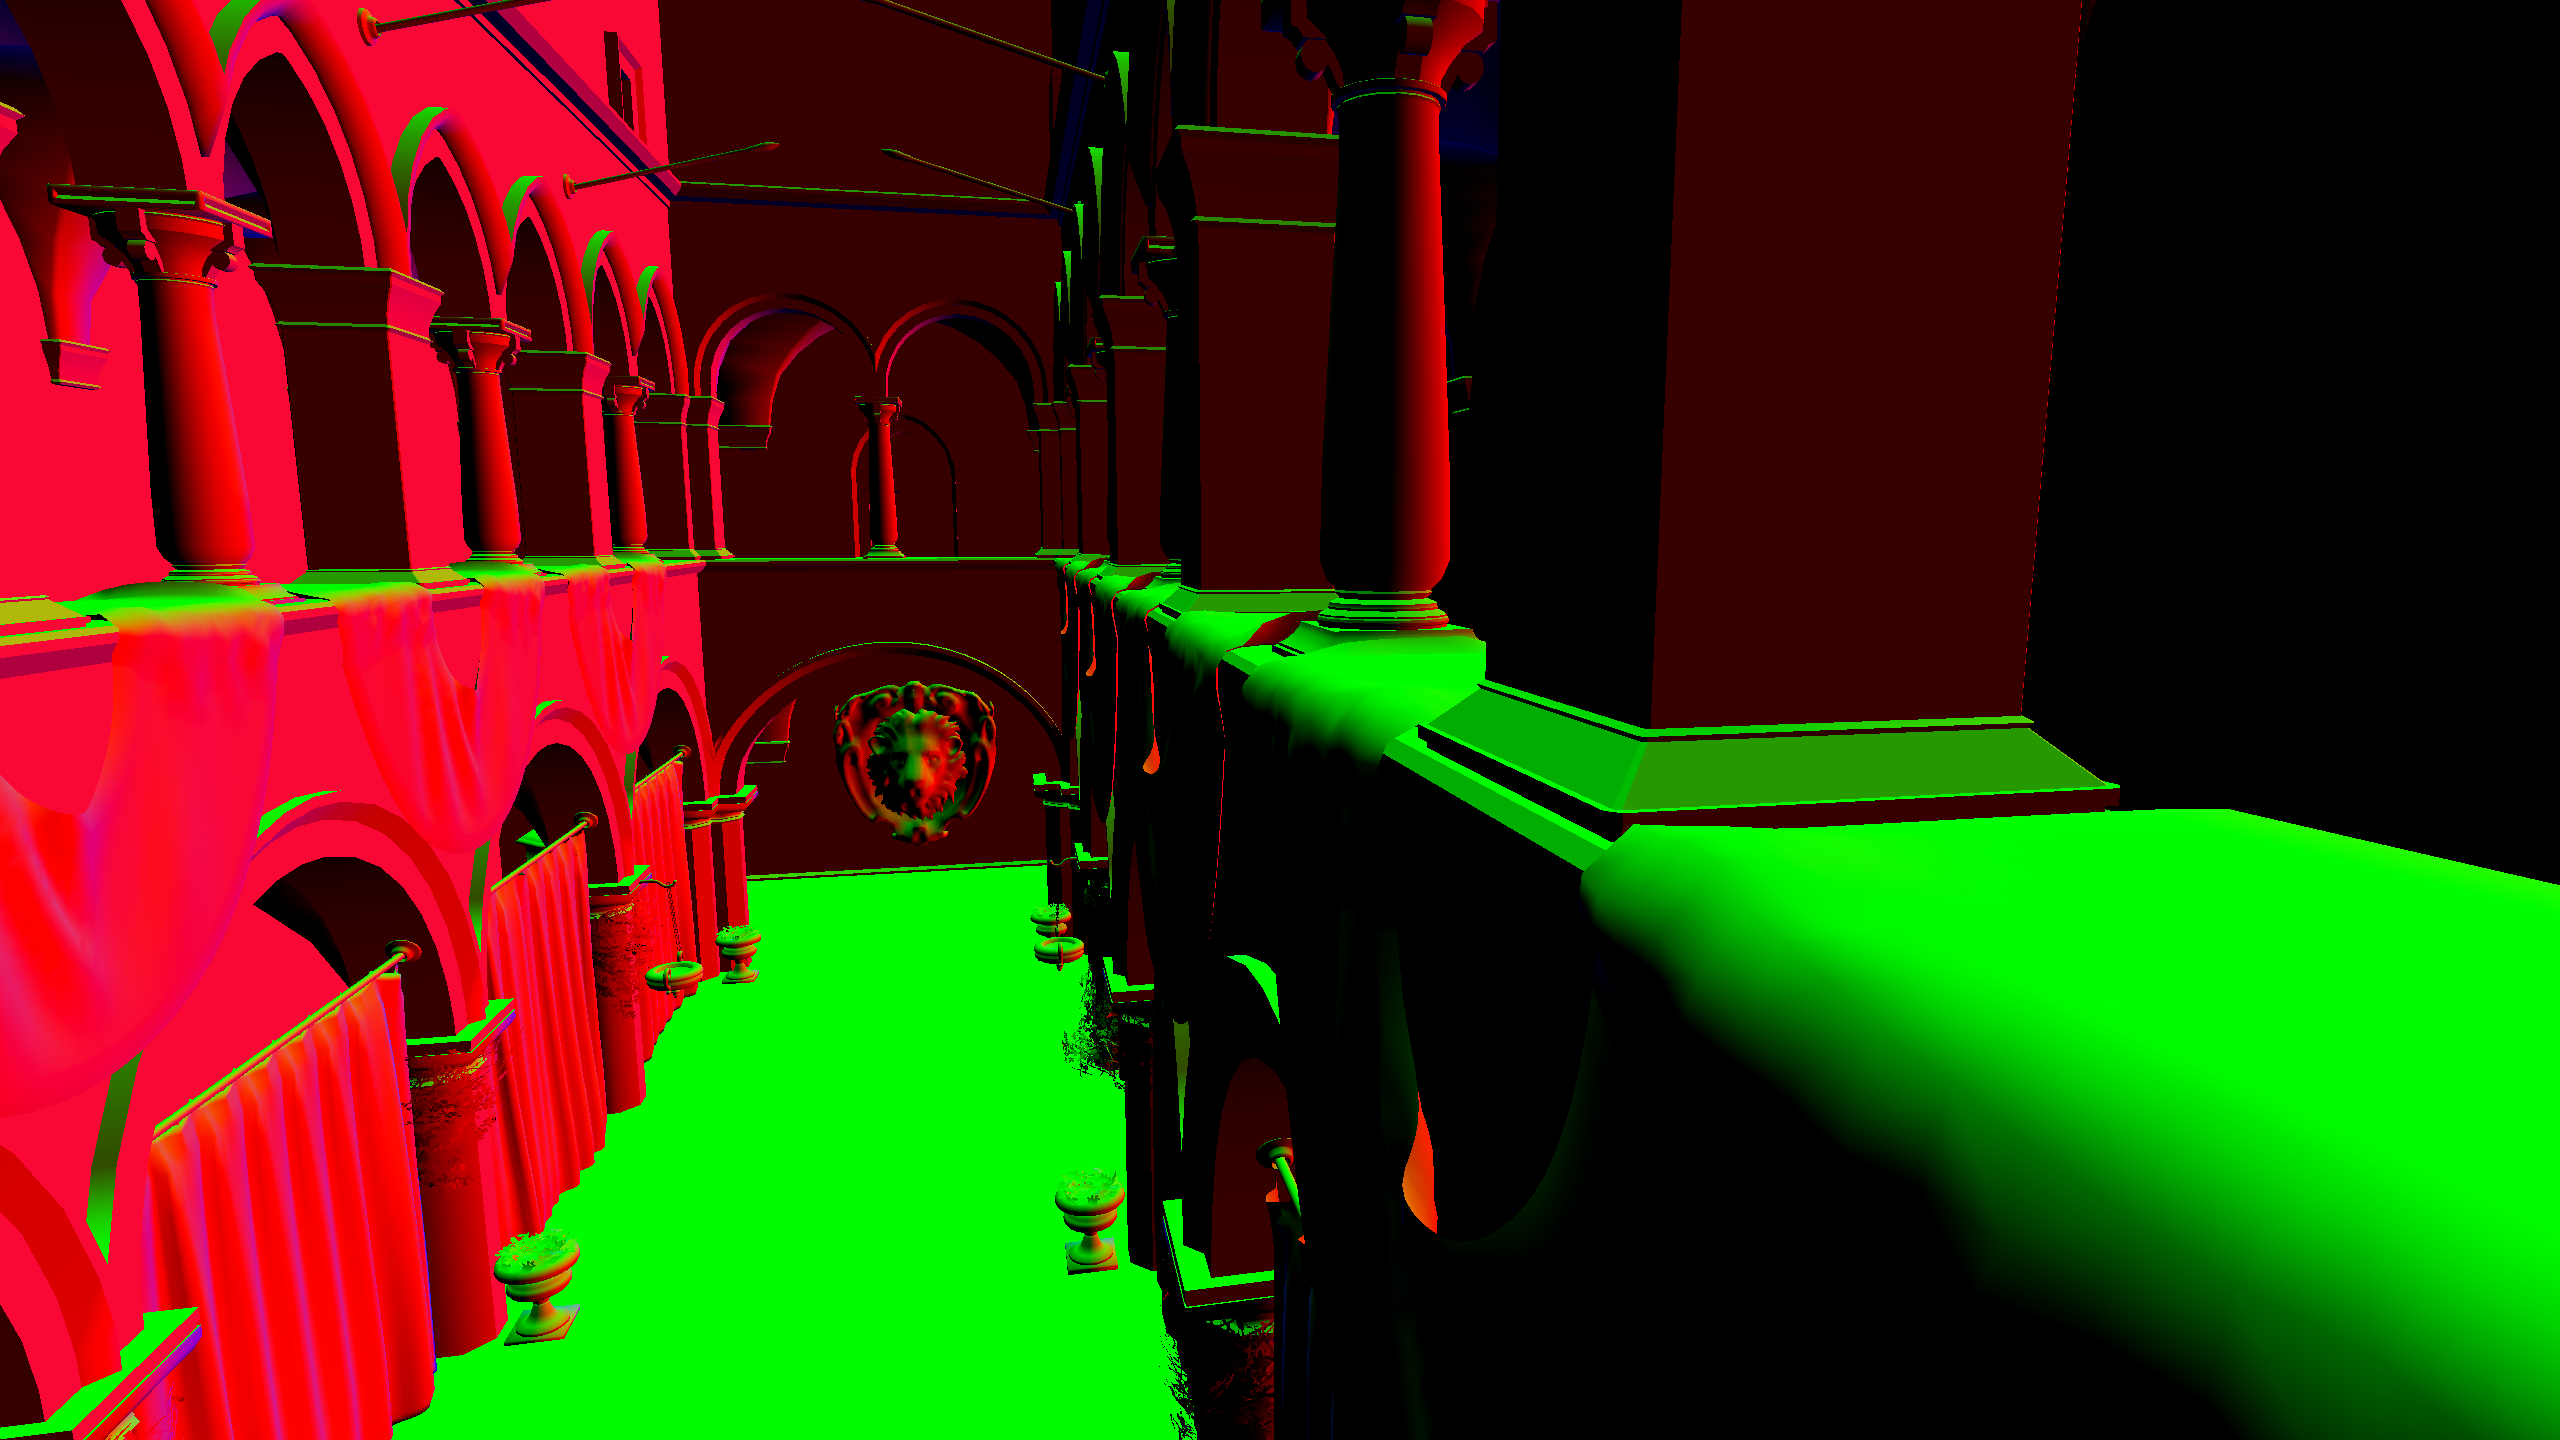
\includegraphics[width=\textwidth]{images/norm.png}
\end{frame}

\begin{frame}
    \frametitle{Применение фильтра Собеля к нормалям}
    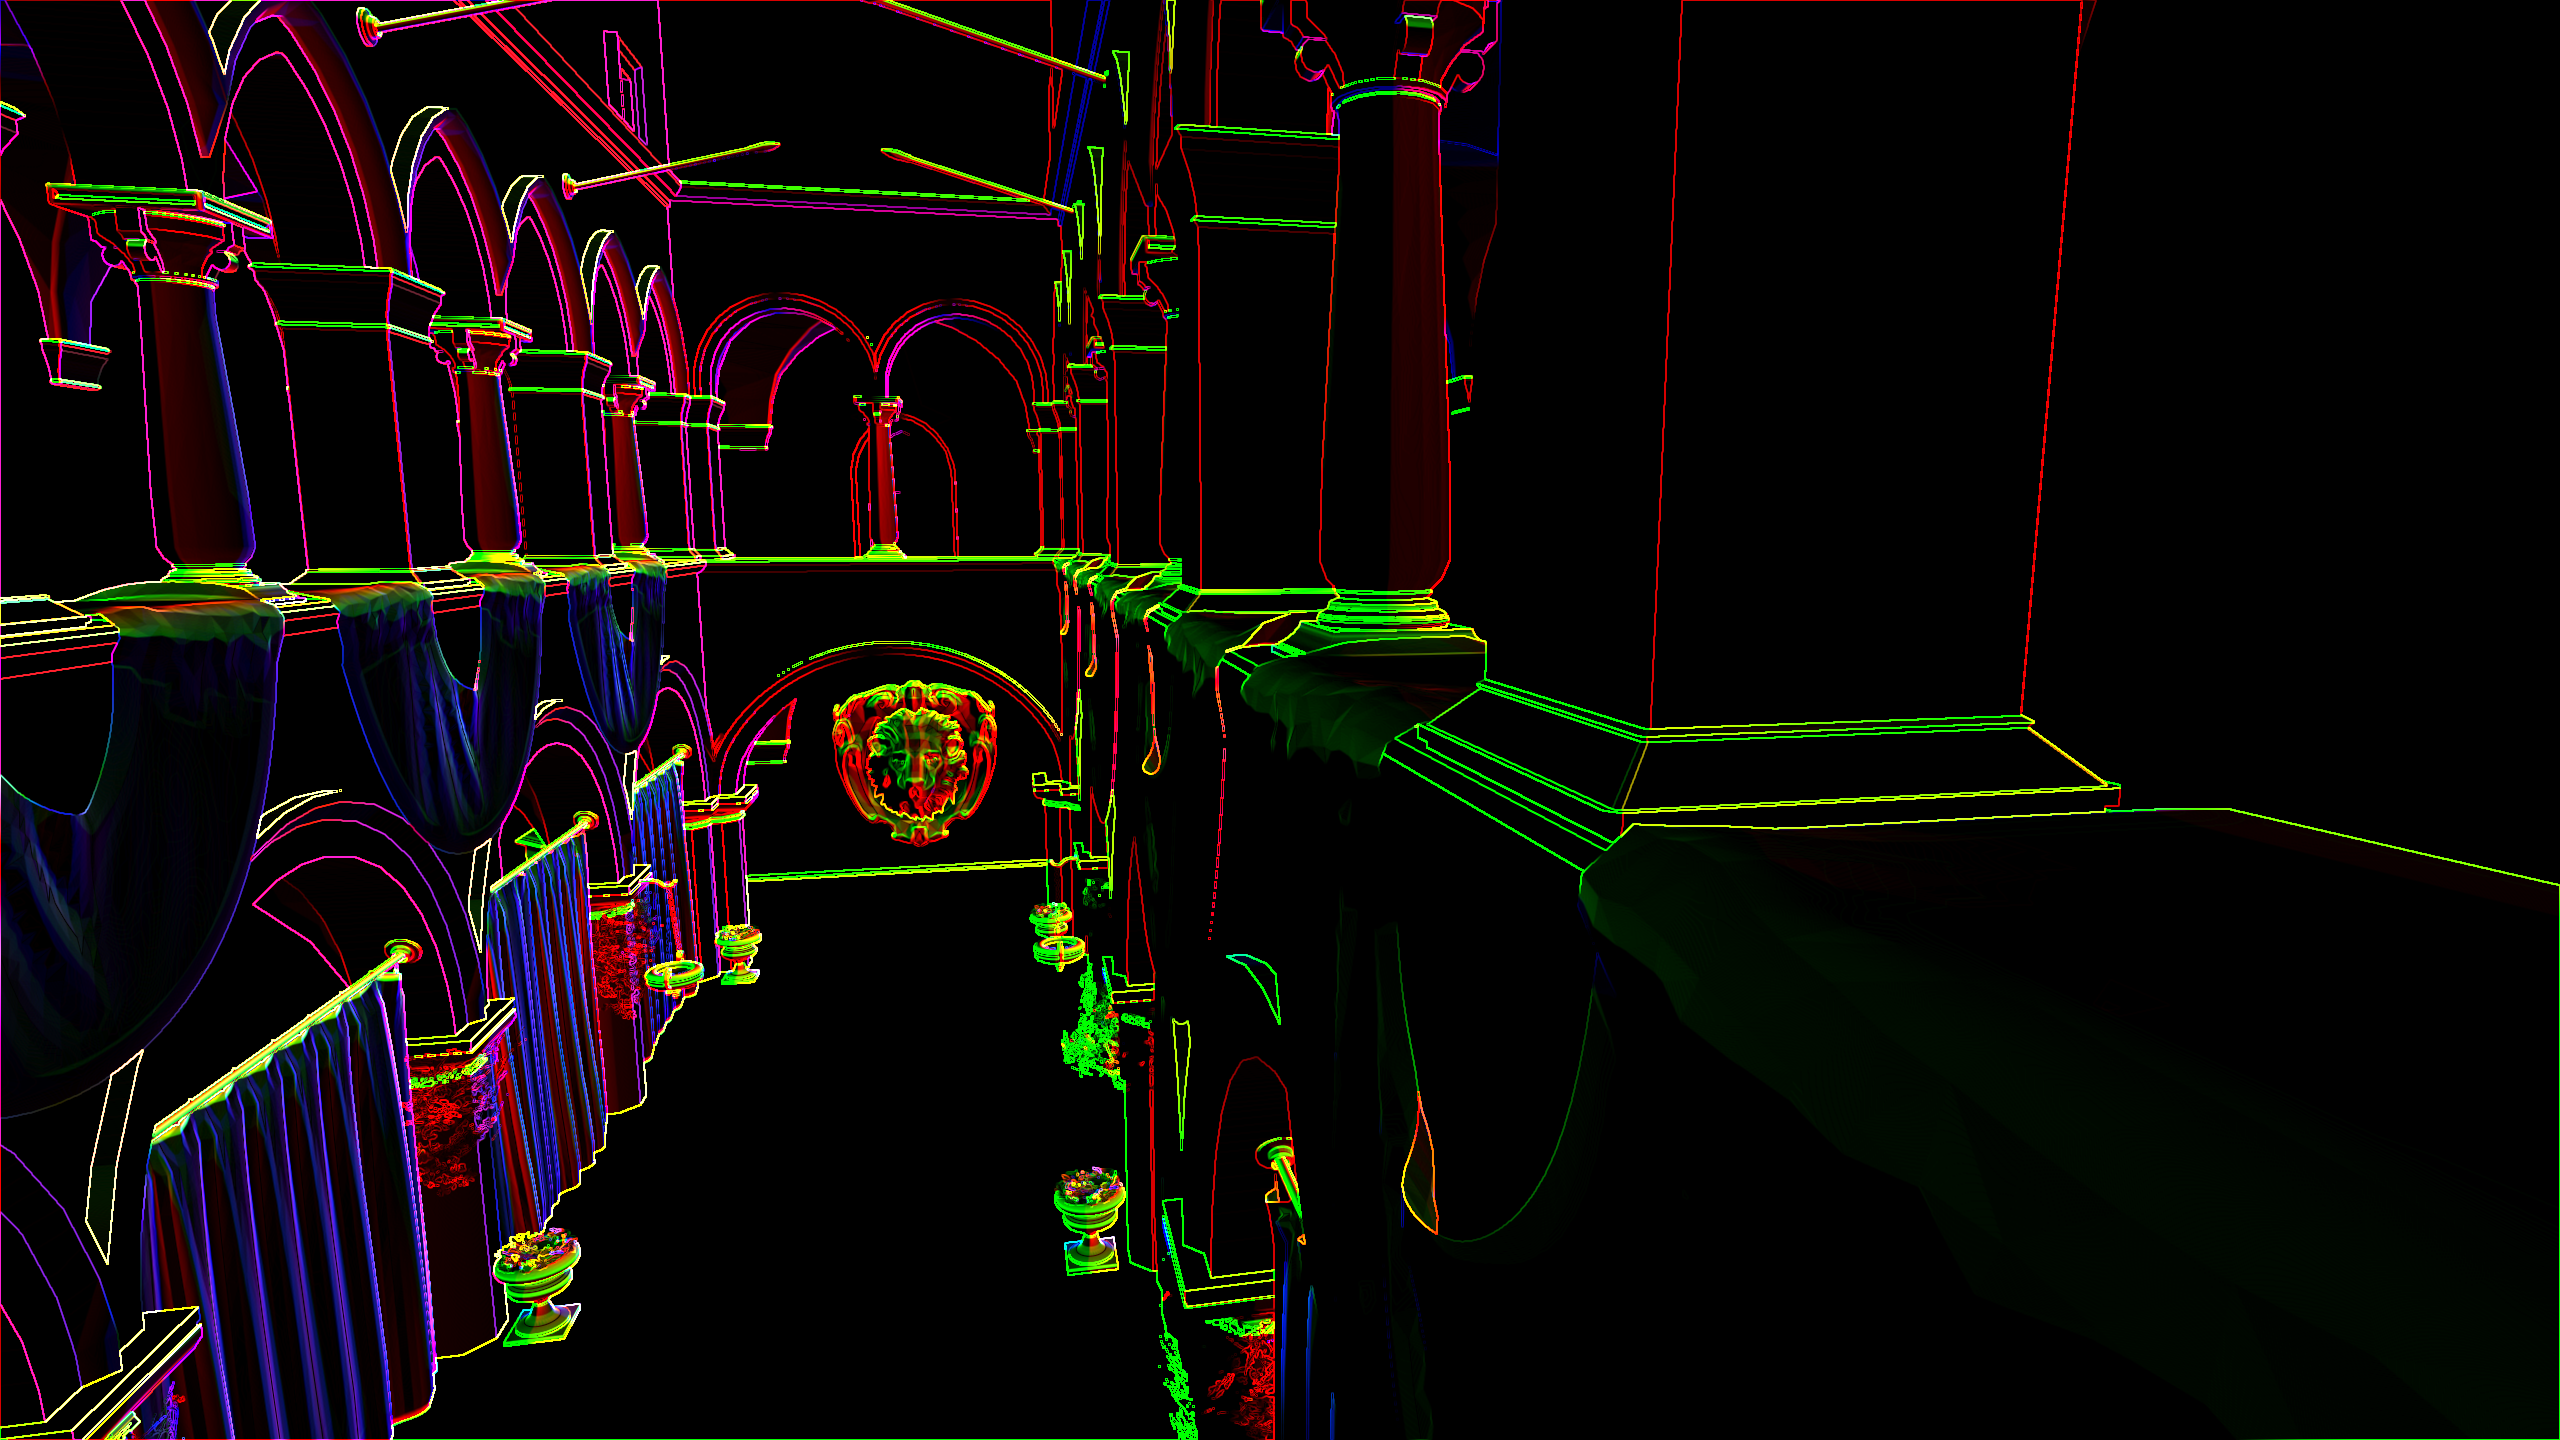
\includegraphics[width=\textwidth]{images/sobel-norm.png}
\end{frame}

\begin{frame}
    \frametitle{Простейшее освещение}
    \includegraphics[width=\textwidth]{images/lighting.png}
\end{frame}

\begin{frame}
    \frametitle{Применение фильтра Собеля к освещению}
    \includegraphics[width=\textwidth]{images/sobel-lighting.png}
\end{frame}
